\documentclass[12pt,twoside]{report}
\usepackage{graphicx}
\usepackage{alphalph}
\usepackage{subcaption}
\usepackage[a5paper,margin=1cm]{geometry}
\renewcommand*{\thesubfigure}{(\arabic{subfigure})}
\begin{document}
\begin{figure}
\centering
\begin{subfigure}[b]{0.20\textwidth}
\centering

\includegraphics[width=\textwidth]{../../trajectories/85.png}
\caption{Id:85}
\end{subfigure}
\begin{subfigure}[b]{0.20\textwidth}
\centering

\includegraphics[width=\textwidth]{../../trajectories/106.png}
\caption{Id:106}
\end{subfigure}
\begin{subfigure}[b]{0.20\textwidth}
\centering

\includegraphics[width=\textwidth]{../../trajectories/174.png}
\caption{Id:174}
\end{subfigure}
\begin{subfigure}[b]{0.20\textwidth}
\centering

\includegraphics[width=\textwidth]{../../trajectories/195.png}
\caption{Id:195}
\end{subfigure}
\begin{subfigure}[b]{0.20\textwidth}
\centering

\includegraphics[width=\textwidth]{../../trajectories/215.png}
\caption{Id:215}
\end{subfigure}
\begin{subfigure}[b]{0.20\textwidth}
\centering
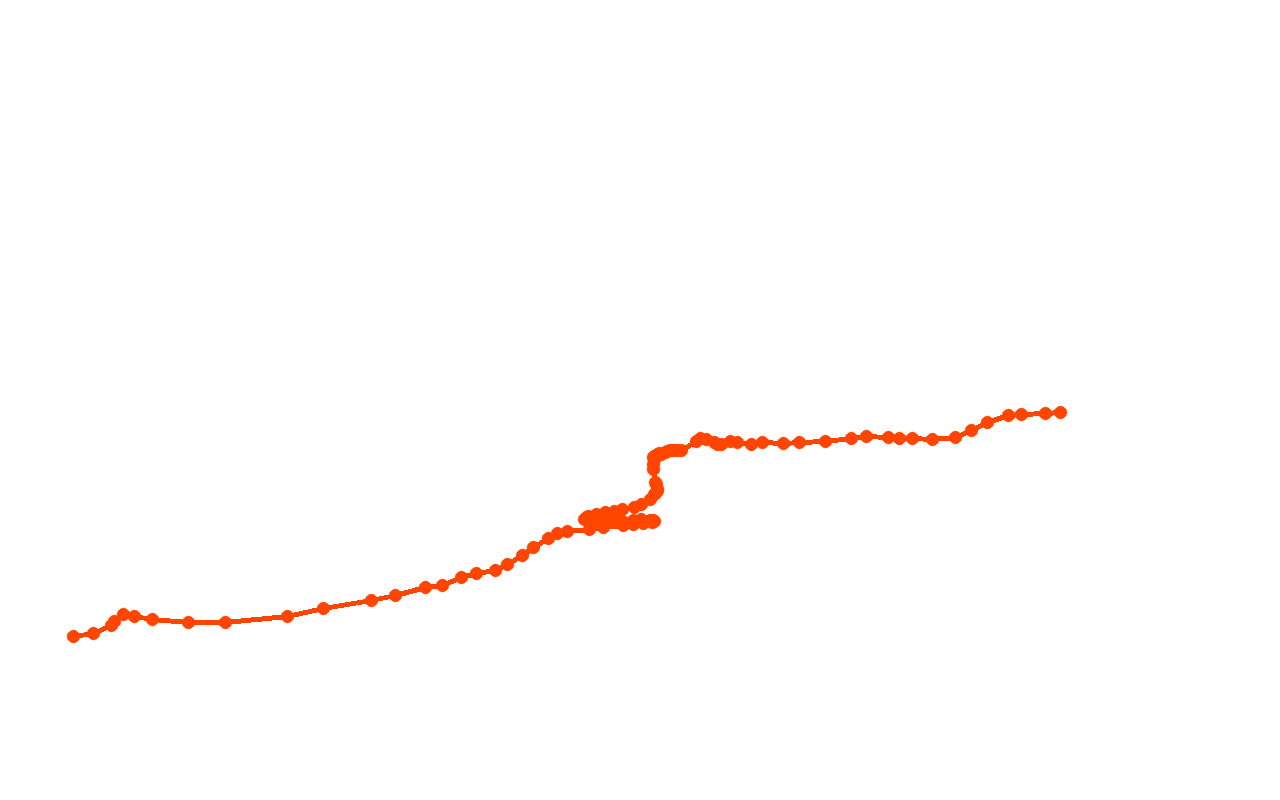
\includegraphics[width=\textwidth]{../../trajectories/828.png}
\caption{Id:828}
\end{subfigure}
\end{figure}
\end{document}